\fancyfoot[RE,LO]{Autor: Julia Gartner}

\section {Mobile Applications} \label {MobileApplications}

\subsection {Einleitung} \label {MAEinleitung}

Eine Mobile Application, oft nur App genannt, ist Software, die auf mobilen Ger�ten verwendet werden kann. Solche Ger�te sind z.B. Smartphones, Tablets oder Smartwatches und haben meistens entweder Android oder iOS als Betriebssystem\cite{reg401}. Generell gibt es viele Anwendungen f�r mobile App wie Kommunikation, E-Commerce und Weiterbildung\cite{reg402}. In unserem Fall hat das Software Interface prim�r die Aufgabe, die mithilfe des EOGs gesammelten Daten f�r den User graphisch darzustellen. Sekund�r gibt es eine Weckerfunktion.

\subsection {Allgemeines zur Mobilapp-Entwicklung} \label {MAAllgemeines}

Wie bereits in Kapitel \ref{MAEinleitung} erw�hnt, sind die meistverbreiteten Betriebssysteme, die die Umgebung f�r Mobile Apps darstellen, iOS und Android mit einem Marktanteil von 99\% im Jahr 2018 in den USA. Mobile Apps f�r diese beiden Betriebssysteme werden jedoch nicht in der selben Sprache geschrieben. F�r Android kann in Java oder Kotlin geschrieben werden, w�hrend f�r iOS Objective-C oder Swift verwendet wird. Das ist in der Praxis oft nicht optimal, da eine Anwendung erstens in zwei verschiedenen Sprachen geschrieben werden muss und zweitens auch zwei verschiedene Anwendungen gewartet werden m�ssen\cite{reg403}. Eine L�sung f�r dieses Problem sind Hybrid Mobile App Development Frameworks. Mit diesen Frameworks k�nnen Apps in einer Sprache geschrieben werden und trotzdem auf verschiedenen Betriebssystemen laufen\cite{reg404}.\\

\begin{figure}[H]
	\centering
		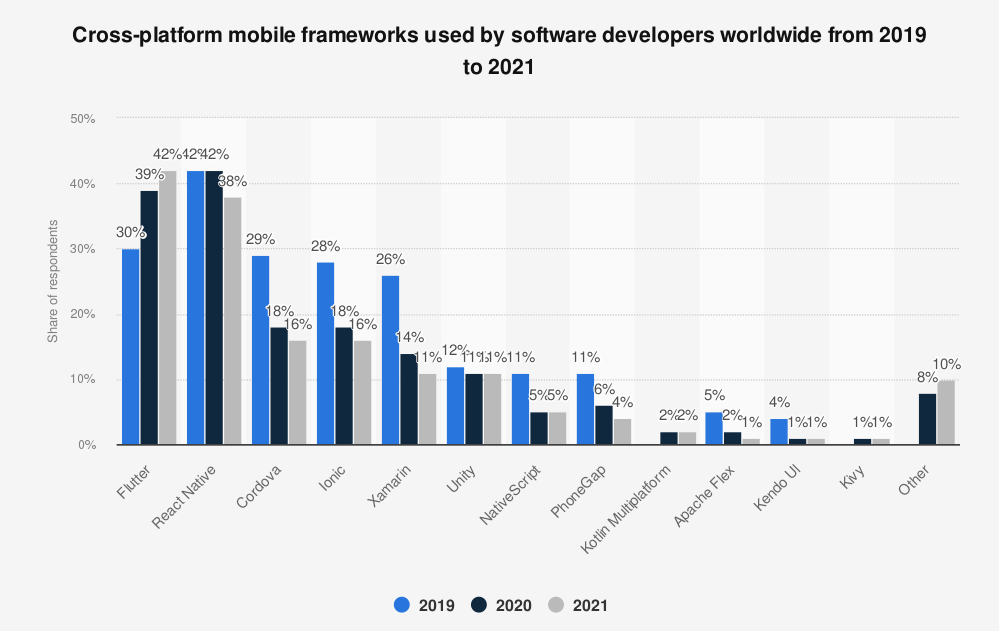
\includegraphics[width=0.9\textwidth]{Gartner/assets/cross_platform_use_statistic.png}
	\caption{Plattform�bergreifende Mobile-Frameworks die von Softwareentwicklern weltweit verwendet werden (2019 bis 2021)\cite{reg405}}
	\label{fig:cross_platform_use_statistic}
\end{figure}

Wie in Abbildung \ref{fig:cross_platform_use_statistic} zu sehen ist, sind die zwei meist verwendeten plattform�bergreifenden Mobile-Frameworks seit 2019 Flutter und React Native, was sich immer weiter absetzt. W�hrend im Jahr 2019 das meistverwendete Framwork noch React Native war, verwenden 2021 die meisten Entwickler bereits Flutter.  \\
React Native und Flutter unterscheiden sich in mehreren Hinsichten. Zum einen wird das React Native-Framework mit JavaScript verwendet, w�hrend ein Flutter-Projekt in Dart geschrieben wird. React Native erreicht die plattformunabh�ngige Anwendung durch eine Br�cke; ein React Native-Projekt in JavaScript auf einem Android-Ger�t z.B. kommuniziert �ber diese Br�cke mit nativen Komponenten des Betriebssystems. Bei Flutter hingegen wird ein Projekt beim Kompilieren von Dart direkt zu einer nativen Sprache �bersetzt, f�r ein Ger�t ist das also nicht zu unterscheiden von einer nativen App\cite{reg406}.

\subsubsection {Entwicklungsumgebung} \label{MAEntwicklungsemgebung}

VSCode, Android Studio Emulator

\subsection {Flussdiagramm} \label {MAFlussdiagramm}

\begin{figure}[H]
	\centering
		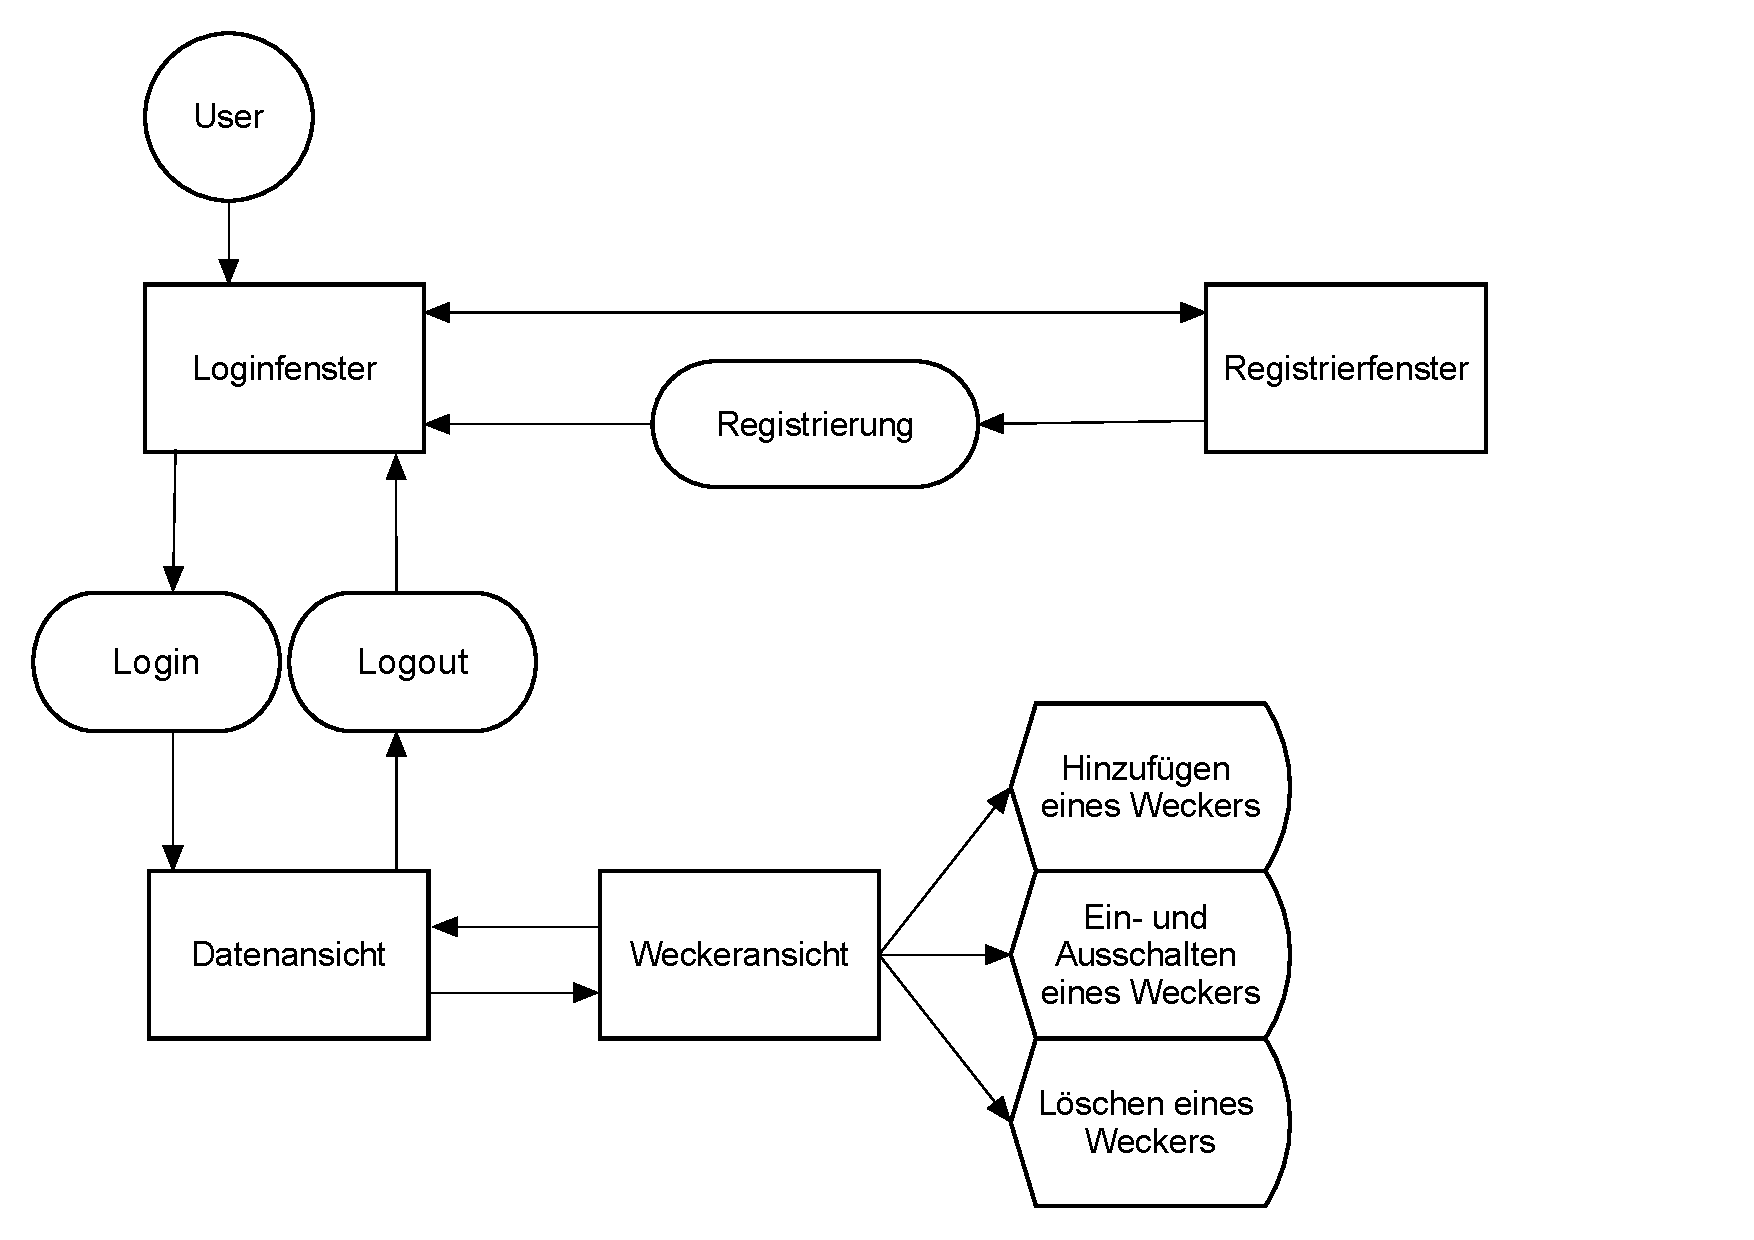
\includegraphics[width=0.9\textwidth]{Gartner/flussdiagramm.pdf}
	\caption{Flussdiagramm der Mobile Application}
	\label{fig:MA_Flussdiagramm}
\end{figure}

\begin{figure}[H]
	\centering
		
\includegraphics[width=0.45\textwidth]{Gartner/buffer.jpg}
	\caption{Loginfenster des GUI}
	\label{fig:MA_Loginfenster}
\end{figure}

\begin{figure}[H]
	\centering
		
\includegraphics[width=0.45\textwidth]{Gartner/buffer.jpg}
	\caption{Registrierfenster des GUI}
	\label{fig:MA_Registrierfenster}
\end{figure}

Der erste Bildschirm ist wie in Abbildung \ref{fig:MA_Flussdiagramm} zu erkennen entweder das Loginfenster oder der Homescreen mit der Datenansicht. Falls man die App zum ersten Mal �ffnet oder sich in der letzten Session abgemeldet hat, ist das in Abbildung \ref{fig:MA_Loginfenster} zu sehende Loginfenster der Startpunkt. Von hier aus kann sich der Benutzer entweder einloggen, wenn er schon einen Account hat, oder zum Registrierfenster, wie in Abbildung \ref{MA_Registrierfenster} gezeigt, wechseln, um sich zu registrieren. Wenn die Registrierung erfolgreich war, wird wieder zum Loginfenster geleitet. Es gibt aber auch die M�glichkeit, ohne Registrierung wieder zum Loginfenster zu wechseln. In beiden F�llen muss der Login im Loginfenster erfolgen, um die Datenansicht zu laden. \\

\begin{figure}[H]
	\centering
		
\includegraphics[width=0.45\textwidth]{Gartner/buffer.jpg}
	\caption{Datenansicht des GUI}
	\label{fig:MA_Datenansicht}
\end{figure}

Im Fall, dass der User sich bereits einmal eingeloggt und in der letzten Session nicht abgemeldet hat, wird direkt die Datenansicht geladen. Hier gibt es, wie in Abbildung \ref{MA_Datenansicht} zu sehen, eine Navigationsleiste am unteren Ende des Bildschirms, mit dem ausgew�hlt werden kann, ob die Daten- oder Weckeransicht gezeigt wird. \\
In der Datenansicht werden alle Messergebnisse der EOG-Messungen eines Benutzers angezeigt. Hier gibt es, abgesehen vom Scrollfeature, keine Interaktionsm�glichkeiten. \\

\begin{figure}[H]
	\centering
		
\includegraphics[width=0.45\textwidth]{Gartner/buffer.jpg}
	\caption{Weckeransicht des GUI}
	\label{fig:MA_Weckeransicht}
\end{figure}

Die Weckeransicht, gezeigt in Abbildung \ref{fig:MA_Weckeransicht}, erm�glicht eine Verwaltung der Weckerfunktion. M�gliche Interaktionen hier sind das Hinzuf�gen oder Entfernen und das Ein- oder Ausschalten eines Weckers. Hinzugef�gte Wecker werden ebenfalls hier angezeigt. \\

\begin{figure}[H]
	\centering
		
\includegraphics[width=0.45\textwidth]{Gartner/buffer.jpg}
	\caption{Logout des GUI}
	\label{fig:MA_Logout}
\end{figure}

Wie bereits in Abbildung \ref{MA_Datenansicht} und \ref{MA_Weckeransicht} zu erkennen, ist links oben in der Ansicht ein Menu Button implementiert. Das dahinterliegende Menu mit der Logout-Funktion ist in Abbildung \ref{MA_Logout} zu sehen. 

%\subsection {Funktionalit�t} \label {}

\subsection {Framework} \label {MAFramework} 

Wie bereits in Kapitel \ref{MAAllgemeines} erw�hnt, wurde f�r dieses Projekt Flutter als Framework gew�hlt. Das hat mehrere Gr�nde, doch zun�chst etwas zur Geschichte von Flutter.\\
Flutter wurde 2016 von Google auf den Markt gebracht. Im Gegensatz zu React Native, das auf einem bereits vorher bestandenen Framework aufgebaut wurde und ein Jahr fr�her auf den Markt gekommen ist, hat Google Flutter neu aufgebaut. Hierbei haben die Entwickler - im Gegensatz zu React Native, das in JavaScript geschrieben wird - Dart als Sprache gew�hlt. Das war allerdings nicht von Anfang an klar, da vor allem zu Beginn JavaScript eigentlich die erste Wahl gewesen w�re\cite{reg406}.\\

\paragraph {Dart} \label{MAFramework_Dart}

Dart wurde urspr�nglich von Google f�r Webdevelopment entwickelt und war als Alternative zu JavaScript angedacht. Da teilweise JavaScript-Standards eingehalten worden sind, gibt es �hnliche Befehle in den beiden Sprachen wie zum Beispiel \glqq async \grqq{}oder \glqq await \grqq. Trotzdem ist die Syntax eher Java-�hnlich aufgebaut\cite{reg417}.\\
Einer der Vorteile von Dart ist, dass die Sprache AOT (ahead of time) und JIT (Just in Time) kompiliert werden kann. Code, der JIT kompiliert wird, ist oft viel langsamer, daf�r ist AOT kompilierter Code nicht plattformunabh�ngig. Code, der JIT kompiliert wird, l�uft in der Dart-VM. Mithilfe davon k�nnen Programme nur teilweise neu kompiliert werden, ohne dass das gesamte Programm neu kompiliert wird. Das erm�glicht eine viel schnellere und angenehmere Entwicklung, da �nderungen im Programm sehr schnell �bertragen und ausgetestet werden k�nnen. Au�erdem erm�glicht es einige Debug-Funktionen. F�r die praktische Anwendung eines Projekts, nach der Entwicklungsphase, kann Dart dann in nativen Code umgewandelt werden\cite{reg417}.\\
Ein weiterer Vorteil, den Dart gegen�ber JavaScript hat, ist ein generational garbage collector.\\
W�hrend Zuteilung und auch das Freigeben von Speicher in Sprachen wie C manuell geregelt werden muss, gibt es daf�r in h�heren Sprachen automatisierte Prozesse, wie zum Beispiel den Garbage Collector (GC). Die Aufgabe eines GCs ist es, unbenutzten Speicher wieder freizugeben. Zu diesem Zweck wird �berpr�ft, welche Objekte nicht mehr referenziert werden und diese dann gel�scht, wie in Abbildung \ref{fig:gr_MAFramework_GC1} zu sehen ist:

\begin{figure}[H]
	\centering
		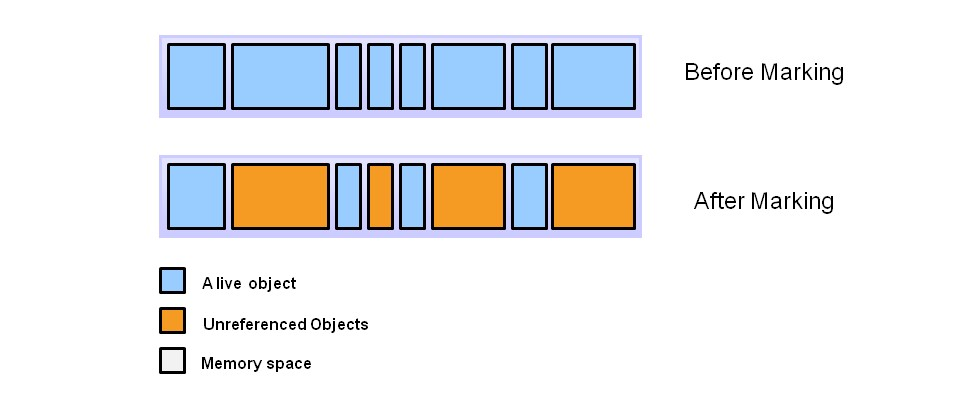
\includegraphics[width=0.9\textwidth]{Gartner/assets/gr_MAFramework_GC1.jpg}
	\caption{Markieren unreferenzierter Objekte\cite{reg419}}
	\label{fig:gr_MAFramework_GC1}
\end{figure}

Es dauert jedoch relativ lang, eine gesamte Anwendung nach referenzierten und nicht-referenzierten Objekten zu durchsuchen. Ein Ansatz, um diesen Prozess schneller zu machen, ist der generational GC. Diese Art von GC baut darauf auf, dass die meisten Objekte sehr nah an ihrere Erstellung wieder collected werden k�nnen, und Objekte, die schon einige Zeit lang bestehen, oft noch l�nger bestehen als neue. Die �berlegung ist also, dass �ltere Objekte nicht mehr so oft auf ihre Referenzierung �berpr�ft werden m�ssen. In Abbildung \ref{fig:gr_MAFramework_GC2} ist ein m�glicher Aufbau eines generational GCs gezeigt:

\begin{figure}[H]
	\centering
		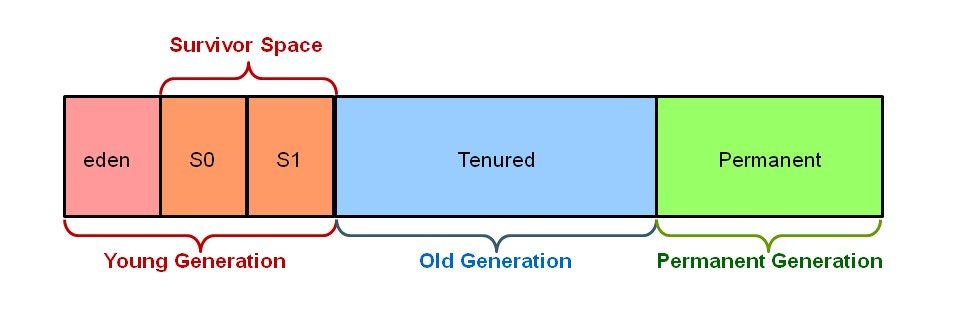
\includegraphics[width=0.9\textwidth]{Gartner/assets/gr_MAFramework_GC2.jpg}
	\caption{verschiedene Generationen des GC\cite{reg419}}
	\label{fig:gr_MAFramework_GC2}
\end{figure}

Neue Objekte kommen hier nach Eden. Bei jedem kleineren GC-Event wird Eden und beide survivor spaces auf aussortierbare Objekte durchsucht. 

\begin{figure}[H]
	\centering
		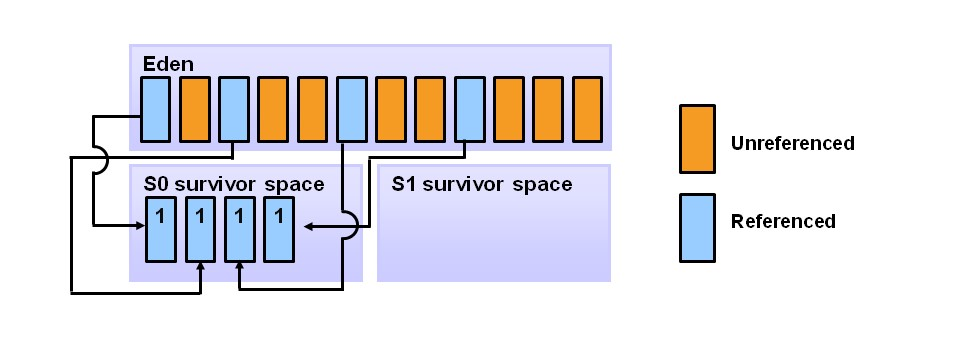
\includegraphics[width=0.9\textwidth]{Gartner/assets/gr_MAFramework_GC3.jpg}
	\caption{Zuteilung der Objekte zu survivor spaces\cite{reg419}}
	\label{fig:gr_MAFramework_GC3}
\end{figure}

Wie in Abbildung \ref{fig:gr_MAFramework_GC3} zu sehen ist, werden referenzierte Objekte in einen der survivor spaces umgelagert und unreferenzierte Objekte als neuer Speicherplatz freigegeben. Bei jedem GC-Event werden auch noch referenzierte Objekte aus einem survivor space in den jeweils anderen geschoben. Wenn diese nun ein gewisses \glqq Alter \grqq{}erreicht haben, werden sie als �ltere Generation festgelegt, und nicht mehr bei jedem GC-Event sondern nur noch gelegentlich �berpr�ft, wie in Abbildung \ref{fig:gr_MAFramework_GC4} gezeigt\cite{reg419}: 

\begin{figure}[H]
	\centering
		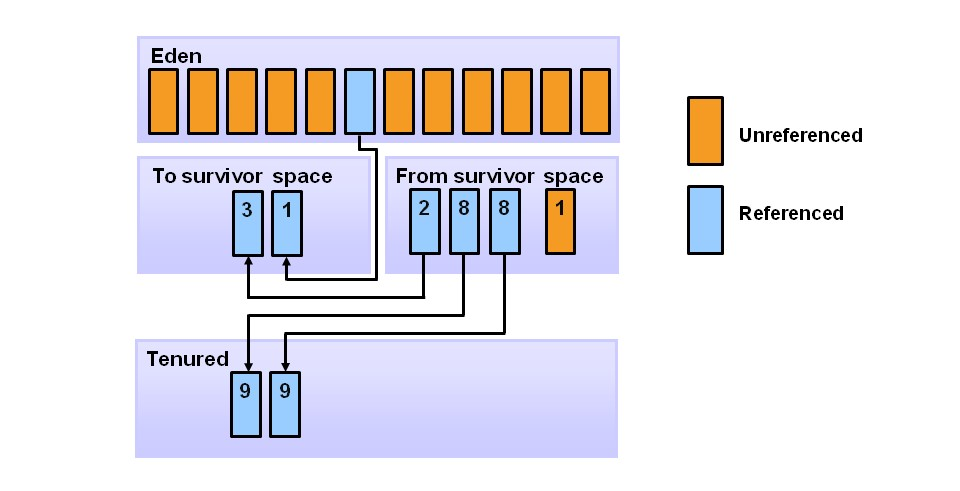
\includegraphics[width=0.9\textwidth]{Gartner/assets/gr_MAFramework_GC4.jpg}
	\caption{Zuteilung der Objekte zu einer �lteren Generation\cite{reg419}}
	\label{fig:gr_MAFramework_GC4}
\end{figure}

Ein weiterer Vorteil des Dart-GC ist, dass GC-Events durchgef�hrt werden, wenn eine App gerade unt�tig ist; das sorgt daf�r, dass die Performance nicht durch das Event gest�rt wird\cite{reg421}.
Da in Flutter potenziell sehr viele Objekte und Widgets erstellt werden, die nach einer kurzen Zeit nicht mehr referenziert werden, ist der GC ein wichtiger Bestandteil.\\
Ein weiterer Vorteil Dart gegen�ber JavaScript ist, dass Dart type-safe ist. Das bedeutet, wenn zum Beispiel eine Variable als Integer definiert wird, diese Variable aber ein String als Wert zugewiesen wird, dann resultiert das in einem compile-time-error (Der Code wird nicht kompiliert). Das hat mehrere Vorteile: Erstens werden somit mit dem Typ verbundene Fehler w�hrend des Kompilierens erkannt. Vor allem bei gro�en Projekten kann es sonst schwierig werden, einen solchen Fehler im Nachhinein zu identifizieren. Weiters ist der Code mit Type-safety einfacher zu lesen und zu erhalten. Ein weiterer Vorteil ist, dass Code mit Type-safety besser AOT-kompiliert werden kann; Kompilieren von nicht type-safe Code ist zwar m�glich, dieser kompilierte Code ist aber weniger effizient\cite{reg422}. \\
Ein weiterer Vorteil Dart gegen�ber JavaScript ist, dass Dart type-safe ist. Das bedeutet, wenn zum Beispiel eine Variable als Integer definiert wird, diese Variable aber ein String als Wert zugewiesen wird, dann resultiert das in einem compile-time-error (Der Code wird nicht kompiliert). Das hat mehrere Vorteile: Erstens werden somit mit dem Typ verbundene Fehler w�hrend des Kompilierens erkannt. Vor allem bei gro�en Projekten kann es sonst schwierig werden, einen solchen Fehler im Nachhinein zu identifizieren. Weiters ist der Code mit Type-safety einfacher zu lesen und zu erhalten. Ein weiterer Vorteil ist, dass Code mit Type-safety besser AOT-kompiliert werden kann; Kompilieren von nicht type-safe Code ist zwar m�glich, dieser kompilierte Code ist aber weniger effizient\cite{reg422}. \\
Ein weiterer Vorteil Darts gegen�ber JavaScript ist, dass es einfach schneller ist. Au�erdem war es auch eine praktische Entscheidung, da das Flutter- und das Dart-Entwicklerteam gut zusammenarbeiten konnten, da beide von Google stammen\cite{reg406}.\\

\paragraph {Flutter Architektur} \label{MAFramework_flutterArchitektur}

Die Architektur Flutters ist wie in Abbildung \ref{fig:gr_MAFramework_archdiagram} dargestellt aufgebaut:

\begin{figure}[H]
	\centering
		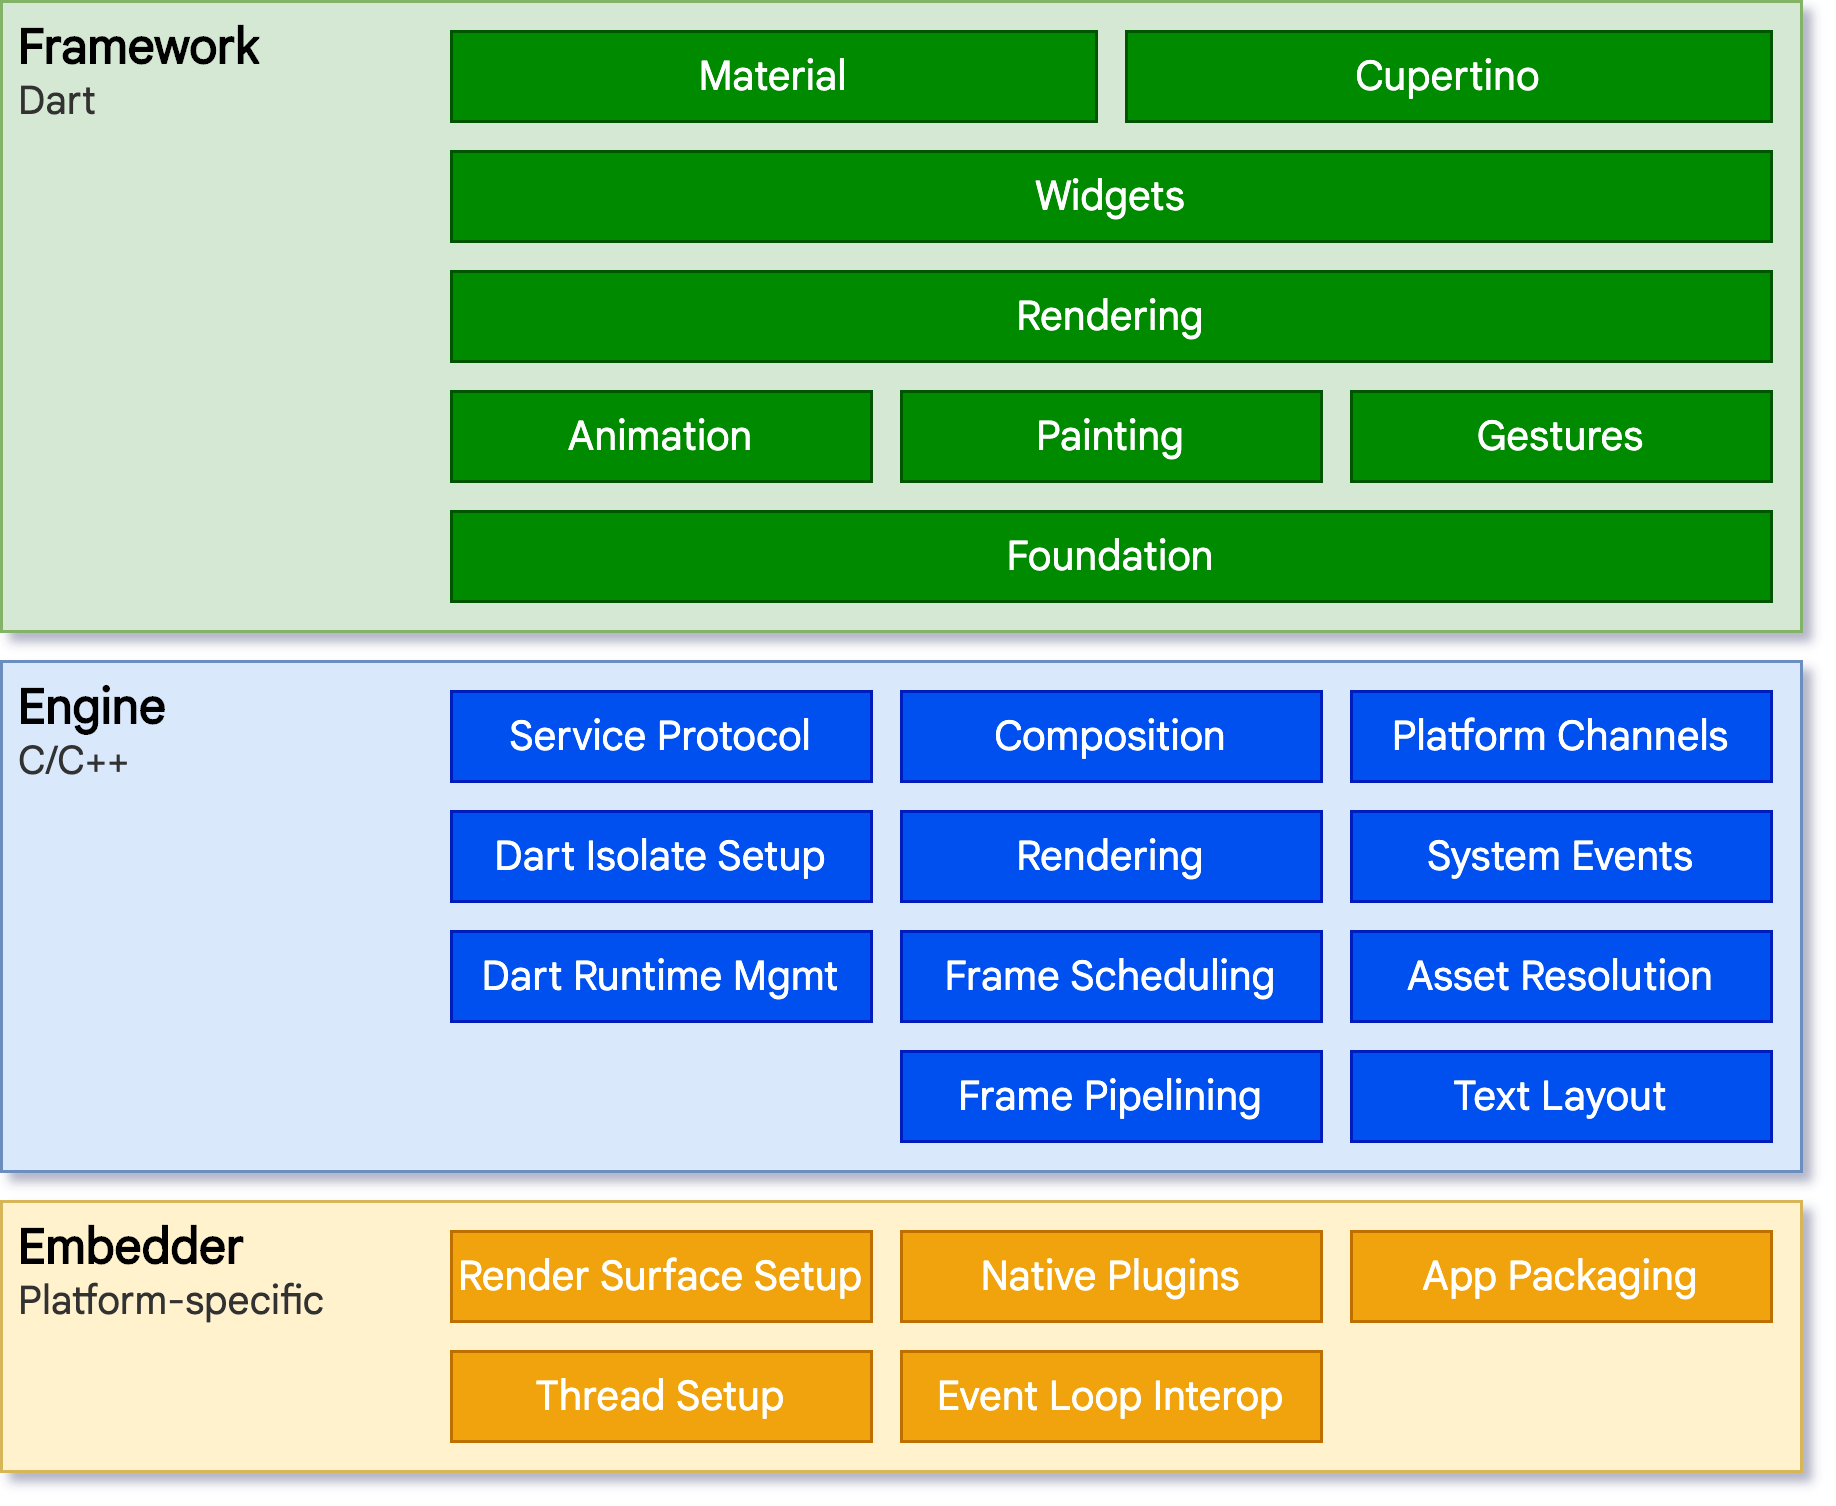
\includegraphics[width=0.9\textwidth]{Gartner/assets/gr_MAFramework_archdiagram.jpg}
	\caption{Diagramm der Architektur Flutters\cite{reg423}}
	\label{fig:gr_MAFramework_archdiagram}
\end{figure}

Das System ist aus verschiedenen Lagen aufgebaut. Eine Lage ist immer von weiter unten liegenden Lagen abh�ngig. Die unterste Lage ist der Embedder. Der Embedder ist die Schnittstelle zwischen dem Betriebssystem und der App. Das ist vor allem wichtig, um Zugang zu Instanzen wie Bildschirm oder Eingabe zu haben. Je nach Betriebssystem ist der Embedder in einer passenden Sprache geschrieben: Java oder C\raisebox{-0.5ex}{++} f�r Android, 


\subsection {Benutzerverwaltung} \label{MABenutzerverwaltung}


Die Benutzerverwaltung ist im Projekt vor allem wichtig, um f�r jeden Benutzer die passenden Datens�tze anzeigen zu k�nnen. Beim �ffnen der App ist der Start immer beim Loginfenster, wo gepr�ft wird, ob der Benutzer bereits eingeloggt ist oder nicht. Zu diesem Zweck wird die User-ID aufgerufen und �berpr�ft, ob sie gr��er als 0 ist. Falls das der Fall ist, wird der Benutzer direkt zum Homescreen weitergeleitet. Falls die User-ID 0 ist, was in der Software als nicht eingeloggt definiert wurde, wird das Loginfenster angezeigt. Wie in Abbildung \ref{fig:MA_Loginfenster} gezeigt, gibt es zwei Textfelder, eines um den Benutzernamen und eines um das Passwort einzugeben. Es gibt eine Reihe von Fehlern, die beim Einloggen auftreten k�nnen: 

\begin{figure}[H]
	\centering
		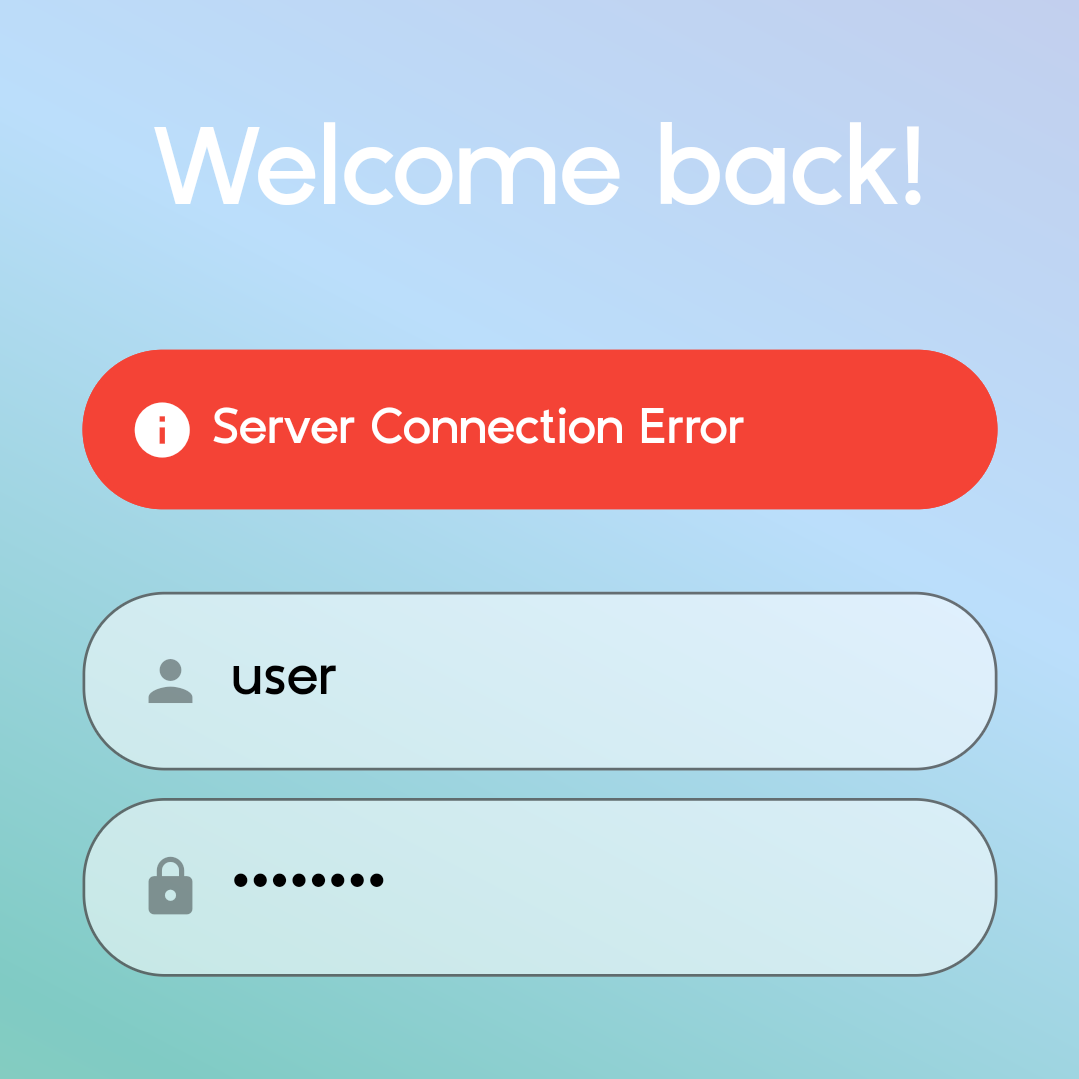
\includegraphics[width=0.4\textwidth]{Gartner/assets/ss_benutzerverwaltung_serverConnectionError.png}
	\caption{Fehlermeldung: \glqq Server Connection Error\grqq}
	\label{fig:ss_benutzerverwaltung_serverConnectionError}
\end{figure}

Die Abbildung \ref{fig:ss_benutzerverwaltung_serverConnectionError} zeigt die Fehlermeldung bei Verbindungsproblemen zum Server. Eine Ursache f�r dieses Problem kann sein, dass entweder der Benutzer oder der Server keine Internetverbindung hat. Diese Fehlermeldung ist in der lokalen Software verankert, es gab also keinen Kontakt zum Server. 

\begin{figure}[H]
	\centering
		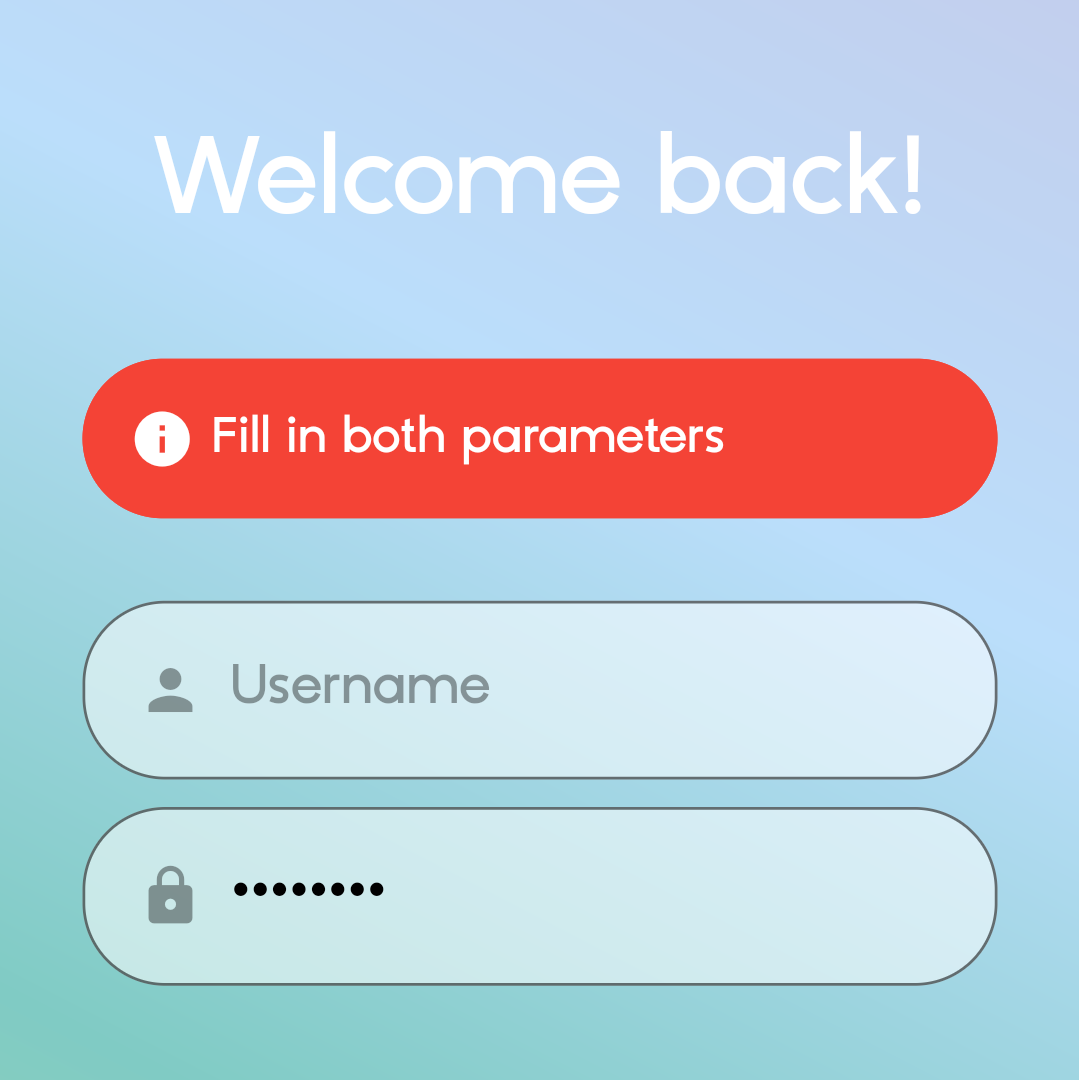
\includegraphics[width=0.4\textwidth]{Gartner/assets/ss_benutzerverwaltung_fillInBothParameters.png}
	\caption{Fehlermeldung: \glqq Fill in both Parameters\grqq}
	\label{fig:ss_benutzerverwaltung_fillInBothParameters}
\end{figure}

Abbildung \ref{fig:ss_benutzerverwaltung_fillInBothParameters} zeigt die Fehlermeldung bei Nichtausf�llen einer oder zwei Textfelder. Diese Fehlermeldung wird von dem Server �bergeben, kann also bei fehlender Internetverbindung gar nicht entstehen. 

\begin{figure}[H]
	\centering
		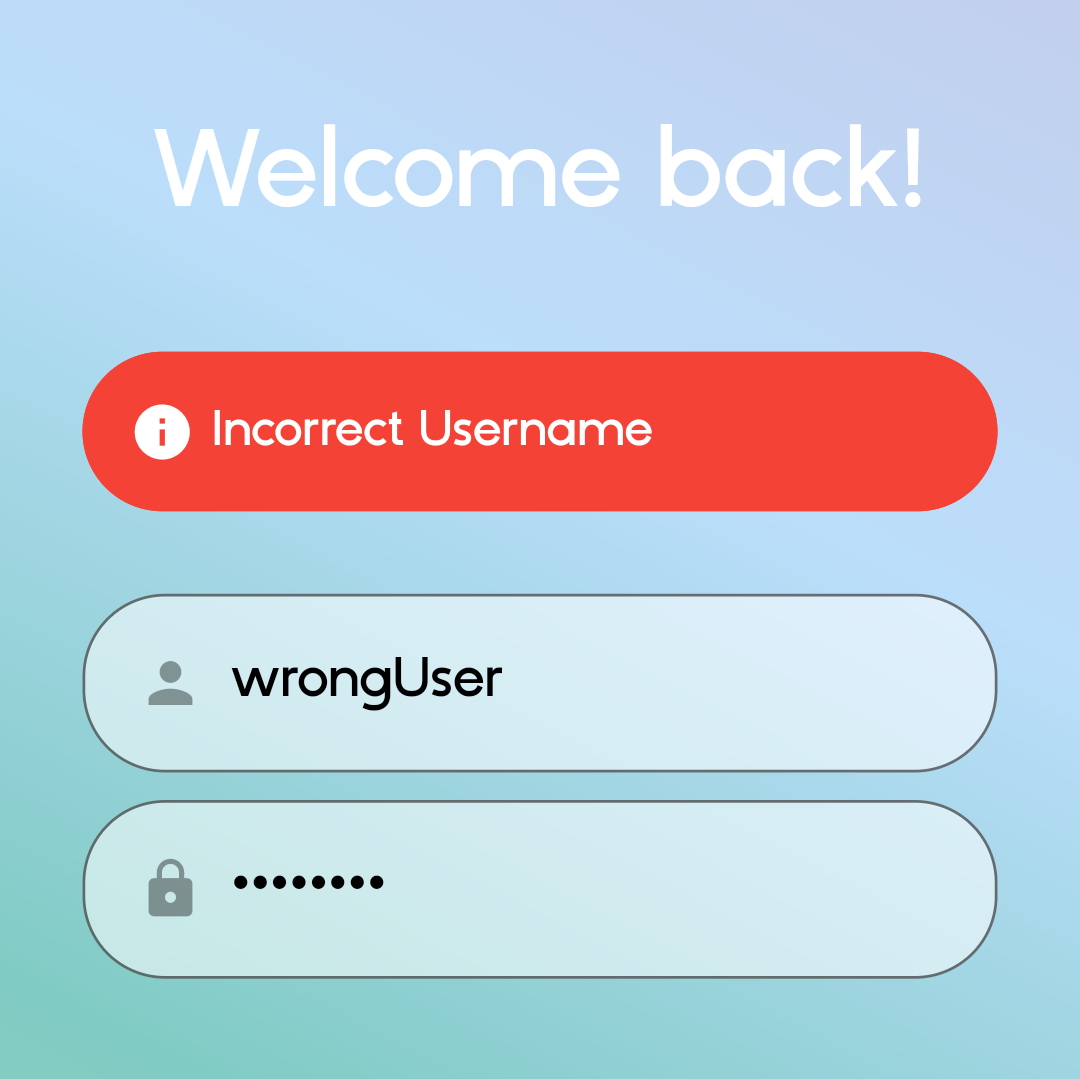
\includegraphics[width=0.4\textwidth]{Gartner/assets/ss_benutzerverwaltung_incorrectUsername.png}
	\caption{Fehlermeldung: \glqq Incorrect Username\grqq}
	\label{fig:ss_benutzerverwaltung_incorrectUsername}
\end{figure}

In Abbildung \ref{fig:ss_benutzerverwaltung_incorrectUsername} ist die Fehlermeldung bei Angabe eines ung�ltigen Usernames zu sehen. Diese Fehlermeldung wird ebenfalls vom Server �bergeben. 

\begin{figure}[H]
	\centering
		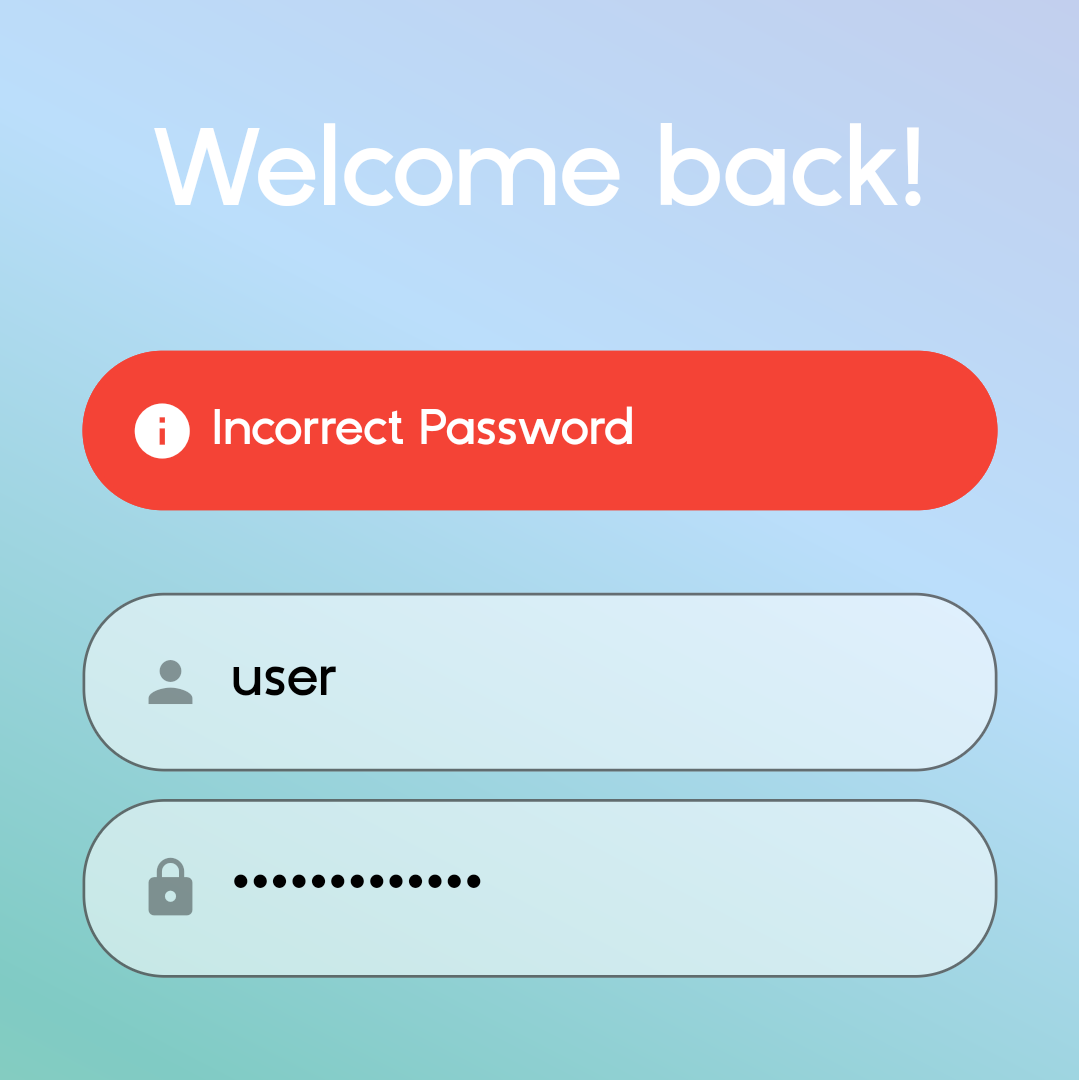
\includegraphics[width=0.4\textwidth]{Gartner/assets/ss_benutzerverwaltung_incorrectPassword.png}
	\caption{Fehlermeldung: \glqq Incorrect Password\grqq}
	\label{fig:ss_benutzerverwaltung_incorrectPassword}
\end{figure}

Abbildung \ref{fig:ss_benutzerverwaltung_incorrectPassword} zeigt die Fehlermeldung bei Angabe eines ung�ltigen Passworts. Wie die zwei eben genannten Fehlermeldungen stammt auch diese vom Server.\\

Falls die Anmeldung allerdings erfolgreich ist, also Verbindung zwischen Server und Client besteht und der Benutzer einen g�ltigen Benutzernamen und Passwort eingibt, wird er zum Homescreen weitergeleitet w�hrend im Hintergrund der Server die User-ID zur�ckgibt, welche dann gespeichert wird. F�r das Auslesen und Speichern dieser Daten gibt es zwei Prinzipien, die wichtig sind: Wie Daten permanent gespeichert werden, und wie die Daten dann �ber den Widget-Baum hinweg aufgerufen werden k�nnen.

\subsubsection {Permanenter Speicher} \label{}

In einem Projekt werden Variablen allerdings nicht prinzipiell permanent gespeichert, sondern gel�scht, wenn die Anwendung geschlossen wird. Das ist bei der Benutzerverwaltung ein Problem, wenn der Benutzer eingeloggt bleiben soll. Wenn Daten also auf einem Ger�t selbst, und nicht auf z.B. einem seperaten Server gespeichert werden sollen, muss daf�r ein Plug-in installiert werden. Eine M�glichkeit hierf�r w�re SQLite, eine kompakte SQL-Datenbank-engine. SQLite wird von vielen Entwicklern verwendet, auch au�erhalb des Flutter-Frameworks\cite{reg415}. \\
W�hrend SQLite gut f�r gr��ere Projekte oder Projekte, die auf ein komplexeres Speichersystem hingewiesen sind geeignet ist, gibt es auch einfacher zu implementeriende L�sungen. Eine davon ist das Package \glqq get\_storage\grqq{}, das in diesem Projekt verwendet wurde. Die Entscheidung wurde aufgrund der einfacheren Implementierung, aber auch wegen der Geschwindigkeit der Klasse getroffen. Tats�chlich ist GetStorage so schnell, dass der Zugriff und die Speicherung in der Klasse als synchrone Abl�ufe stattfinden (mehr dazu in Kapitel \ref{MADataFetching_AsyncFunctions})\cite{reg416}. \\
In der Software wird GetStorage f�r die Benutzerverwaltung und die Weckerfunktion ben�tigt.

\subsubsection {State Management} \label{}

Es gibt zwei verschiedene Arten von Widgets in Flutter: Stateless und Stateful Widgets. Stateful Widgets sind Widgets, die sich ver�ndern k�nnen, wenn z.B. Daten dargestellt werden oder der Benutzer mit dem Widget interagieren kann. Stateless Widgets hingegen sind Widgets, die sich nie ver�ndern\cite{reg407}.\\
State ist Information, die ermittelt werden kann, w�hrend ein Widget gebaut wird und sich auch �ndern kann. Beim Entwickeln einer App in Flutter muss also darauf geachtet werden, dass beim Auftreten solcher �nderungen ein Widget auch neu aufgebaut wird, da die dahinterliegenden Informationen sich sonst ge�ndert haben, aber nicht das Widget selbst. Das kann mit Methoden wie z.B. setState geregelt werden\cite{reg408}. Hier k�nnen aber Probleme entstehen, wenn State �ber verschiedene Klassen hinweg weitergegeben werden muss; Dies kann zwar mit �bergabeparametern gel�st werden, aber auch hier bleibt das genannte Problem bestehen und vor allem bei gr��eren Projekten ist die L�sung bei weitem nicht ideal.\\
Im Internet k�nnen viele Klassen gefunden werden, die State Management vereinfachen sollen. Eine der Basisklassen ist die InheritedWidget class. Die Logik hinter der Klasse ist, dass State im Baum nach unten vererbt werden kann, sich die verkn�pften Widgets sich bei einer �nderung des States in einem dar�berliegenden Widget also auch neu aufbauen\cite{reg409}. 
F�r das Projekt Sleepanalyzer wurde die Klasse provider zusammen mit ChangeNotifier verwendet, was einer der popul�rsten Ans�tze ist. Klassen k�nnen als ChangeNotifier Klasse angelegt werden. Andere Klassen k�nnen dann subscriben, um bei �nderungen verst�ndigt zu werden. Die Klasse Provider sorgt daf�r, dass State nicht durch den ganzen Widgetbaum weitergegeben werden muss, sondern direkt zu einem bestimmten Widget weitergegeben werde kann. Dazu muss allerdings eine Liste in einem Widget �ber einem Provider und dem Widget, in dem der State gebraucht wird angelegt sein\cite{410}.

\subsubsection {Implementierung} \label{}

\begin{figure}[H]
	\centering
		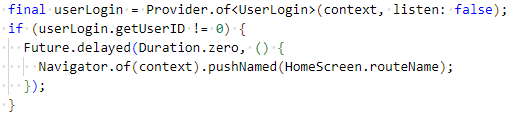
\includegraphics[width=0.9\textwidth]{Gartner/assets/code_benutzerverwaltung_1.png}
	\caption{Quellcodeausschnitt zur Benutzerverwaltung}
	\label{fig:code_benutzerverwaltung_1}
\end{figure}



\subsection {Graphische Darstellung der Daten} \label{}

syncfusion flutter charts

\subsubsection {Data Fetching} \label{MADataFetching}

Da bei der Messung des EOGs die Daten direkt vom Mikrocontroller zu einem Server geschickt werden und dort auf einer Datenbank gespeichert werden, m�ssen diese zur Ansicht der Daten in der App zuerst vom Server angefragt werden. Wenn in der App zur Datenansicht gewechselt wird, entweder vom Loginfenster oder von der Weckeransicht, wird von einem Widget eine Funktion aufgerufen, in der ein Post-Request an den Server gestellt wird. Der body dieses Requests enth�lt die momentan g�ltige User-ID. Am Server werden alle Daten, die zu dieser ID vorhanden sind gesammelt und ebenfalls in einem Post-Request im JSON-Format zur�ckgesendet. Diese Daten werden dann in der App weiter verwertet. Im Folgenden werden alle einzelnen Schritte n�her erl�utert. 

\paragraph{Async functions} \label{MADataFetching_AsyncFunctions}

Da Vorg�nge wie das Warten auf eine Antwort des Servers nach dem Senden eines POST-Requests lange dauern, w�re es nicht gut, wenn alle anderen Vorg�nge w�hrenddessen blockiert sind. Deshalb gibt es Unterscheidungen zwischen synchronen und asynchronen Vorg�ngen. Bei synchronen Operationen wird ein Schritt nach dem anderen abgehandelt, w�hrend bei asynchronen Operationen w�hrenddessen andere Operationen durchgef�hrt werden k�nnen. Die Klasse, die f�r asynchrone Vorg�nge im Flutter-Framework verwendet wird ist die Future\flq T\frq{} Klasse. Ein \glqq future\grqq{} ist eine Instanz der Klasse Future und ist das Ergebniss einer asynchronen Funktion. Wenn nun eine asynchrone Funktion aufgerufen wird, wird ein unvollst�ndeiges future zur�ckgegeben. Dieses future wartet auf den wirklichen Wert, der von der Funktion zur�ckgegeben wird (falls eine Funktion einen R�ckgabewert hat). \\
Dies sorgt daf�r, dass w�hrend auf die Antwort des Servers gewartet werden muss, alle anderen Vorg�nge in der App weiter bestehen bleiben.

\paragraph{HTTP Requests} \label{}

Es gibt eine Reihe von Requests, die im HTTP-Protokoll angef�hrt sind und oft in zur Datenvermittelung verwendet werden. Zwei der h�ufigsten davon sind der POST- und der GET-Request. Diese beiden unterscheiden sich in mehreren Hinsichten. Wie der Name es annehmen l�sst ist ein GET-Request urspr�nglich f�r die Anfrage an einen Server nach Daten und ein POST-Request f�r das Vermitteln von Daten an den Server gedacht. Dies muss in der Praxis allerdings nicht immer eingehalten werden\cite{reg413}. \\
Einer der wichtigsten Unterschiede ist, dass bei einem GET-Request die gesamte Anfrage im Header eines Requests angef�hrt ist, und somit die L�nge auch an die maximale URL-L�nge eines Browsers angepasst werden muss; Ein GET-Request kann also f�r Internet Explorer zum Beispiel maximal 2.048 Zeichen, abz�glich der Anzahl der Zeichen des Pfads, betragen. \\
Bei einem POST-Request ist das nicht der Fall, da der Inhalt eines POST-Requests nicht im header, sondern im Message-body angef�hrt wird\cite{reg413},\cite{reg414}. \\

\paragraph {Implementierung} \label{MADataFetching_Implementierung}

\begin{figure}[H]
	\centering
		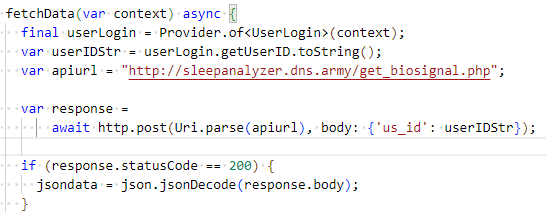
\includegraphics[width=0.9\textwidth]{Gartner/assets/async_post_json.png}
	\caption{Quellcodeausschnitt zur Kommunikation mit dem Server}
	\label{fig:async_post_json}
\end{figure}

In Abbildung \ref{fig:async_post_json} ist die Funktion zur Anfrage und Erhaltung der Daten vom Server zu sehen. Zuerst wird ein POST-Request geschickt, in dessen body die Benutzer-ID festgelegt ist. Die Antwort des Servers erfolgt im JSON-Format und muss dekodiert werden. 



\subsubsection {Weckerfunktion} \label{MAWeckerfunktion}

syncfusion flutter charts

\subsubsection {Design} \label{}

Material Design






